\documentclass[journal,12pt,twocolumn]{IEEEtran}
%
\usepackage{setspace}
\usepackage{gensymb}
%\doublespacing
\singlespacing

%\usepackage{graphicx}
%\usepackage{amssymb}
%\usepackage{relsize}
\usepackage[cmex10]{amsmath}
%\usepackage{amsthm}
%\interdisplaylinepenalty=2500
%\savesymbol{iint}
%\usepackage{txfonts}
%\restoresymbol{TXF}{iint}
%\usepackage{wasysym}
\usepackage{amsthm}
%\usepackage{iithtlc}
\usepackage{mathrsfs}
\usepackage{txfonts}
\usepackage{stfloats}
\usepackage{bm}
\usepackage{cite}
\usepackage{cases}
\usepackage{subfig}
%\usepackage{xtab}
\usepackage{longtable}
\usepackage{multirow}
%\usepackage{algorithm}
%\usepackage{algpseudocode}
\usepackage{enumitem}
\usepackage{mathtools}
\usepackage{steinmetz}
\usepackage{tikz}
\usepackage{circuitikz}
\usepackage{verbatim}
\usepackage{tfrupee}
\usepackage[breaklinks=true]{hyperref}
%\usepackage{stmaryrd}
\usepackage{tkz-euclide} % loads  TikZ and tkz-base
\usetkzobj{all}
\usetikzlibrary{calc,math}
\usepackage{listings}
    \usepackage{color}                                            %%
    \usepackage{array}                                            %%
    \usepackage{longtable}                                        %%
    \usepackage{calc}                                             %%
    \usepackage{multirow}                                         %%
    \usepackage{hhline}                                           %%
    \usepackage{ifthen}                                           %%
  %optionally (for landscape tables embedded in another document): %%
    \usepackage{lscape}     
\usepackage{multicol}
\usepackage{chngcntr}
%\usepackage{enumerate}

%\usepackage{wasysym}
%\newcounter{MYtempeqncnt}
\DeclareMathOperator*{\Res}{Res}
%\renewcommand{\baselinestretch}{2}
\renewcommand\thesection{\arabic{section}}
\renewcommand\thesubsection{\thesection.\arabic{subsection}}
\renewcommand\thesubsubsection{\thesubsection.\arabic{subsubsection}}

\renewcommand\thesectiondis{\arabic{section}}
\renewcommand\thesubsectiondis{\thesectiondis.\arabic{subsection}}
\renewcommand\thesubsubsectiondis{\thesubsectiondis.\arabic{subsubsection}}

% correct bad hyphenation here
\hyphenation{op-tical net-works semi-conduc-tor}
\def\inputGnumericTable{}                                 %%

\lstset{
%language=C,
frame=single, 
breaklines=true,
columns=fullflexible
}
%\lstset{
%language=tex,
%frame=single, 
%breaklines=true
%}

\begin{document}
%


\newtheorem{theorem}{Theorem}[section]
\newtheorem{problem}{Problem}
\newtheorem{proposition}{Proposition}[section]
\newtheorem{lemma}{Lemma}[section]
\newtheorem{corollary}[theorem]{Corollary}
\newtheorem{example}{Example}[section]
\newtheorem{definition}[problem]{Definition}
%\newtheorem{thm}{Theorem}[section] 
%\newtheorem{defn}[thm]{Definition}
%\newtheorem{algorithm}{Algorithm}[section]
%\newtheorem{cor}{Corollary}
\newcommand{\BEQA}{\begin{eqnarray}}
\newcommand{\EEQA}{\end{eqnarray}}
\newcommand{\define}{\stackrel{\triangle}{=}}

\bibliographystyle{IEEEtran}
%\bibliographystyle{ieeetr}


\providecommand{\mbf}{\mathbf}
\providecommand{\pr}[1]{\ensuremath{\Pr\left(#1\right)}}
\providecommand{\qfunc}[1]{\ensuremath{Q\left(#1\right)}}
\providecommand{\sbrak}[1]{\ensuremath{{}\left[#1\right]}}
\providecommand{\lsbrak}[1]{\ensuremath{{}\left[#1\right.}}
\providecommand{\rsbrak}[1]{\ensuremath{{}\left.#1\right]}}
\providecommand{\brak}[1]{\ensuremath{\left(#1\right)}}
\providecommand{\lbrak}[1]{\ensuremath{\left(#1\right.}}
\providecommand{\rbrak}[1]{\ensuremath{\left.#1\right)}}
\providecommand{\cbrak}[1]{\ensuremath{\left\{#1\right\}}}
\providecommand{\lcbrak}[1]{\ensuremath{\left\{#1\right.}}
\providecommand{\rcbrak}[1]{\ensuremath{\left.#1\right\}}}
\theoremstyle{remark}
\newtheorem{rem}{Remark}
\newcommand{\sgn}{\mathop{\mathrm{sgn}}}
\providecommand{\abs}[1]{\left\vert#1\right\vert}
\providecommand{\res}[1]{\Res\displaylimits_{#1}} 
\providecommand{\norm}[1]{\left\lVert#1\right\rVert}
%\providecommand{\norm}[1]{\lVert#1\rVert}
\providecommand{\mtx}[1]{\mathbf{#1}}
\providecommand{\mean}[1]{E\left[ #1 \right]}
\providecommand{\fourier}{\overset{\mathcal{F}}{ \rightleftharpoons}}
%\providecommand{\hilbert}{\overset{\mathcal{H}}{ \rightleftharpoons}}
\providecommand{\system}{\overset{\mathcal{H}}{ \longleftrightarrow}}
	%\newcommand{\solution}[2]{\textbf{Solution:}{#1}}
\newcommand{\solution}{\noindent \textbf{Solution: }}
\newcommand{\cosec}{\,\text{cosec}\,}
\providecommand{\dec}[2]{\ensuremath{\overset{#1}{\underset{#2}{\gtrless}}}}
\newcommand{\myvec}[1]{\ensuremath{\begin{pmatrix}#1\end{pmatrix}}}
\newcommand{\mydet}[1]{\ensuremath{\begin{vmatrix}#1\end{vmatrix}}}
%\numberwithin{equation}{section}
%\numberwithin{equation}{subsection}
%\numberwithin{problem}{section}
%\numberwithin{definition}{section}
\makeatletter
\@addtoreset{figure}{problem}
\makeatother

\let\StandardTheFigure\thefigure
\let\vec\mathbf
%\renewcommand{\thefigure}{\theproblem.\arabic{figure}}
\renewcommand{\thefigure}{\theproblem}
%\setlist[enumerate,1]{before=\renewcommand\theequation{\theenumi.\arabic{equation}}
%\counterwithin{equation}{enumi}


%\renewcommand{\theequation}{\arabic{subsection}.\arabic{equation}}

\def\putbox#1#2#3{\makebox[0in][l]{\makebox[#1][l]{}\raisebox{\baselineskip}[0in][0in]{\raisebox{#2}[0in][0in]{#3}}}}
     \def\rightbox#1{\makebox[0in][r]{#1}}
     \def\centbox#1{\makebox[0in]{#1}}
     \def\topbox#1{\raisebox{-\baselineskip}[0in][0in]{#1}}
     \def\midbox#1{\raisebox{-0.5\baselineskip}[0in][0in]{#1}}

\vspace{3cm}

\title{Solution For Problem 8.1.26 }
\author{Yogesh Choudhary}
%\title{
%	\logo{Matrix Analysis throughe  Octave}{\begin{center}\includegraphics[scale=.24]{tlc}\end{center}}{}{HAMDSP}
%}


% paper title
% can use linebreaks \\ within to get better formatting as desired
%\title{Matrix Analysis through Octave}
%
%
% author names and IEEE memberships
% note positions of commas and nonbreaking spaces ( ~ ) LaTeX will not break
% a structure at a ~ so this keeps an author's name from being broken across
% two lines.
% use \thanks{} to gain access to the first footnote area
% a separate \thanks must be used for each paragraph as LaTeX2e's \thanks
% was not built to handle multiple paragraphs
%

%\author{<-this % stops a space
%\thanks{}}
%}
% note the % following the last \IEEEmembership and also \thanks - 
% these prevent an unwanted space from occurring between the last author name
% and the end of the author line. i.e., if you had this:
% 
% \author{....lastname \thanks{...} \thanks{...} }
%                     ^------------^------------^----Do not want these spaces!
%
% a space would be appended to the last name and could cause every name on that
% line to be shifted left slightly. This is one of those "LaTeX things". For
% instance, "\textbf{A} \textbf{B}" will typeset as "A B" not "AB". To get
% "AB" then you have to do: "\textbf{A}\textbf{B}"
% \thanks is no different in this regard, so shield the last } of each \thanks
% that ends a line with a % and do not let a space in before the next \thanks.
% Spaces after \IEEEmembership other than the last one are OK (and needed) as
% you are supposed to have spaces between the names. For what it is worth,
% this is a minor point as most people would not even notice if the said evil
% space somehow managed to creep in.



% The paper headers
%\markboth{Journal of \LaTeX\ Class Files,~Vol.~6, No.~1, January~2007}%
%{Shell \MakeLowercase{\textit{et al.}}: Bare Demo of IEEEtran.cls for Journals}
% The only time the second header will appear is for the odd numbered pages
% after the title page when using the twoside option.
% 
% *** Note that you probably will NOT want to include the author's ***
% *** name in the headers of peer review papers.                   ***
% You can use \ifCLASSOPTIONpeerreview for conditional compilation here if
% you desire.




% If you want to put a publisher's ID mark on the page you can do it like
% this:
%\IEEEpubid{0000--0000/00\$00.00~\copyright~2007 IEEE}
% Remember, if you use this you must call \IEEEpubidadjcol in the second
% column for its text to clear the IEEEpubid mark.



% make the title area
\maketitle

\newpage

%\tableofcontents

\bigskip

\renewcommand{\thefigure}{\theenumi}
\renewcommand{\thetable}{\theenumi}
%\renewcommand{\theequation}{\theenumi}
\numberwithin{equation}{subsection}

%\begin{abstract}
%%\boldmath
%In this letter, an algorithm for evaluating the exact analytical bit error rate  (BER)  for the piecewise linear (PL) combiner for  multiple relays is presented. Previous results were available only for upto three relays. The algorithm is unique in the sense that  the actual mathematical expressions, that are prohibitively large, need not be explicitly obtained. The diversity gain due to multiple relays is shown through plots of the analytical BER, well supported by simulations. 
%
%\end{abstract}
% IEEEtran.cls defaults to using nonbold math in the Abstract.
% This preserves the distinction between vectors and scalars. However,
% if the journal you are submitting to favors bold math in the abstract,
% then you can use LaTeX's standard command \boldmath at the very start
% of the abstract to achieve this. Many IEEE journals frown on math
% in the abstract anyway.

% Note that keywords are not normally used for peerreview papers.
%\begin{IEEEkeywords}
%Cooperative diversity, decode and forward, piecewise linear
%\end{IEEEkeywords}



% For peer review papers, you can put extra information on the cover
% page as needed:
% \ifCLASSOPTIONpeerreview
% \begin{center} \bfseries EDICS Category: 3-BBND \end{center}
% \fi
%
% For peerreview papers, this IEEEtran command inserts a page break and
% creates the second title. It will be ignored for other modes.
%\IEEEpeerreviewmaketitle

\begin{abstract}
This document includes different problems and solution on geometry from trigonometry and  linear algebra.It also provides the imformation about the python and latex codes of figures.
\end{abstract}

Download all python codes from 
%
\begin{lstlisting}
svn co svn co https://github.com/yogi13995/yogesh_training/tree/master/Geometry/triangle2/codes
\end{lstlisting}
%
and latex-tikz codes from 
%
\begin{lstlisting}
svn co https://github.com/yogi13995/yogesh_training/tree/master/Geometry/triangle2/figures
\end{lstlisting}
%


\section{Problem}
\renewcommand{\theequation}{\theenumi}
\begin{enumerate}[label=\arabic*.,ref=\thesubsection.\theenumi]
\numberwithin{equation}{enumi}
\item In a cricket match, a batswoman hits a boundary 6 times out of 30 balls she plays. Find the probability that she did not hit a boundary.
\end{enumerate}
%In right triangle ABC, right angled at C, M is
%the mid-point of hypotenuse AB. C is joined to
%M and produced to a point D such that DM =
%CM. Point D is joined to point B. Show that
%
%\begin{enumerate}[label = (\alph*)]
%\item $\triangle  AMC  \cong   \triangle  BMD $
%\item $\triangle DBC $ is a right angle.
%\item $\triangle  DBC  \cong  \triangle  ABC $
%\item $CM = \frac{1}{2} AB$
%\end{enumerate}
\section{Construction}

%\renewcommand{\thefigure}{\theenumi.\arabic{figure}}
\begin{figure}[!ht]
\centering
\resizebox{\columnwidth}{!}{\renewcommand{\theequation}{\theenumi}
\begin{enumerate}[label=\thesection.\arabic*.,ref=\thesection.\theenumi]
\numberwithin{equation}{enumi}
\item  Find the centre and radius of the circle 
\begin{align}
x^2+y^2+8x+10y-8 = 0
\label{eq:circ_basic}
\end{align}
\solution
\eqref{eq:circ_basic} can be expressed as 
\begin{align}
\vec{x}^T\vec{x}+ 2\myvec{4 & 5}\vec{x} -8 = 0
\end{align}
which is of the form \eqref{eq:conic_quad_form} with
\begin{align}
\label{eq:circ_basic_uf}
\vec{u} = \myvec{4\\5}, f = -8
\end{align}
From  Table \ref{table:conics}, the center and radius are given by 
\begin{align}
\vec{c} = -\vec{u} = \myvec{-4\\-5},
r = \sqrt{\norm{u}^2-f} = 7
\end{align}
\item Find the equation of a circle which passes through the points $\vec{P} = \myvec{2\\-2}$ and $\vec{Q} = \myvec{3\\4}$ and whose centre lies on the line  
%\cite{eleven}
\begin{align}
\label{eq:circ_ex1_line}
\myvec{1 & 1} \vec{x} = 2
\end{align}
\solution From \eqref{eq:conic_quad_form} and Table \ref{table:conics}, the equation of a circle can be expressed as
\begin{align}
\label{eq:circ_conic}
\vec{x}^T\vec{x}-2\vec{c}^T\vec{x}+f = 0
\end{align}
where $\vec{c}$ is the centre.
Substituting the given points in 
\eqref{eq:circ_conic} and using 
\eqref{eq:circ_ex1_line}, the following equations are obtained
\begin{align}
2\myvec{2 & -2}\vec{c} -  f &= 8
\\
2\myvec{3 & 4}\vec{c} -  f &= 25
\\
\myvec{1 & 1}\vec{c}  &= 2
\end{align}
which can be expressed as the matrix equation
\begin{align}
\myvec{
1 & 1 & 0
\\
4 & -4 & -1 
\\ 
6 & 8 & -1  
}
\myvec{\vec{c}\\f} = \myvec{2\\8\\25}
\end{align}
Row reducing the augmented matrix
\begin{align}
\myvec{
1 & 1 & 0 & 2
\\
4 & -4 & -1 & 8
\\ 
6 & 8 & -1  & 25
}
\\
\xleftrightarrow[R_3 \leftarrow R_3 -6R_1]{R_2 \leftarrow -R_2+4R_1}
\myvec{
1 & 1 & 0 & 2
\\
0 & 8 & 1 & 0
\\ 
0 & 2 & -1  & 13
}
\\
\xleftrightarrow[R_3 \leftarrow -\frac{4R_3 -R_2}{2}]{R_1 \leftarrow 8R_1-R_3}
\myvec{
8 & 0 & -1 & 16
\\
0 & 8 & 1 & 0
\\ 
0 & 0 & 5  & -52
}
\\
\xleftrightarrow[R_2 \leftarrow \frac{5R_2 -R_3}{4}]{R_1 \leftarrow \frac{5R_1+R_3}{4}}
\myvec{
10 & 0 & 0 & 7
\\
0 & 10 & 0 & 13
\\ 
0 & 0 & 5  & -52
}
\end{align}
Thus, 
\begin{align}
\vec{c} &= \frac{1}{10}\myvec{7\\13}
\\
f &=-\frac{52}{5}
\end{align}
which give the desired equation of the circle.
From Table \ref{table:conics},
%
\begin{align}
 r =  \sqrt{\norm{\vec{c}}^2-f} = \frac{1}{10}\sqrt{1258}
\end{align}
Fig. \ref{fig:CircOr}	verifies the above results.

\begin{figure}[!ht]
\centering
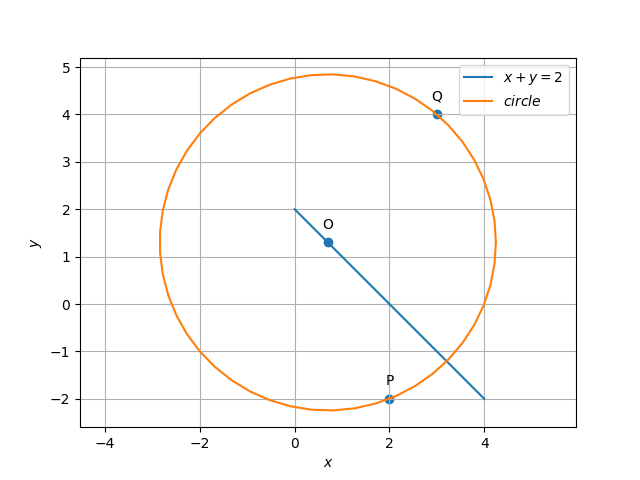
\includegraphics[width=\columnwidth]{./figs/circex/CircOr.eps}
\caption{Circle passing through $\myvec{2\\-2},\myvec{3\\4}$. Center is on line $\myvec{1 & 1}\vec{x}=2$. }
\label{fig:CircOr}	
\end{figure}

\item 
Find the points on the curve  
%\cite{twelve_one}
\begin{align}
x^2+y^2-2x-3 = 0
\label{eq:circle_tangent_prob}
\end{align}
at which the tangents are parallel to the $x$-axis.
\\
\solution \eqref{eq:circle_tangent_prob} can be expressed as
\begin{align}
\vec{x}^T\vec{x}+\myvec{-2 & 0}\vec{x}-3 &= 0
\label{eq:circle_tangent_prob_vec}
\\
\implies \vec{V} = \vec{I}, \vec{u} = \myvec{-1 \\ 0}, f = -3
\label{eq:circle_tangent_prob_uf}
\end{align}
From Table \ref{table:conics}, the centre and radius are
\begin{align}
\vec{c} = -\vec{u} = \myvec{-1 \\ 0}, r =\sqrt{\norm{\vec{u}}^2-f} = 2
\end{align}
$\because$ the tangents are parallel to the $x$-axis, their direction and normal vectors are respectively,
\begin{align}
\vec{m} = \myvec{1\\0},
\vec{n} = \myvec{0\\1}.
\end{align}
From Table \ref{table:conics},
\begin{align}
\kappa = \pm \sqrt{\frac{\vec{u}^T\vec{u}-f}{\vec{n}^T\vec{n}}} = \pm \sqrt{\frac{4}{1}} = \pm 2
\end{align}
and the desired points of contact are 
\begin{align}
\vec{q}_1, \vec{q}_2 = \myvec{1\\0}\pm 2\myvec{0\\1} =  
\myvec{1 \\  2},
\myvec{1 \\  -2}
\end{align}
%
Fig. \ref{fig:CircOr}	verifies the above results.
\begin{figure}[!ht]
\centering
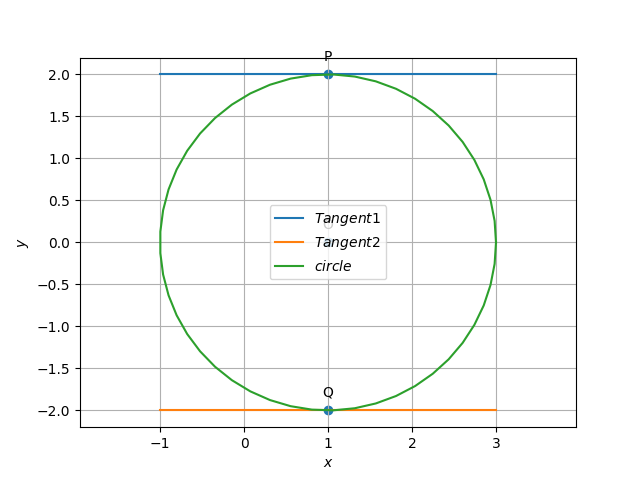
\includegraphics[width=\columnwidth]{./figs/circex/CircTangent.eps}
\caption{Tangents are parallel to the $x$-axis. }
\label{fig:CircTangent}	
\end{figure}

\end{enumerate}
}
\caption{}
\label{fig:8.5.16_circle_latex}	
\end{figure}
%
%
%\renewcommand{\thefigure}{\theenumi}
%
\item {\em Construction: }In Fig. \ref{fig:8.5.16_circle_latex} the known parameters are
%\label{}
\\
%
%\solution From the given information, 
%$\triangle ABC$ are 
\begin{align}
\vec{O} &= \myvec{0\\0} ,
\\
\vec{A} &= \myvec{r\\0} ,
\label{eq:8.5.16_constr_a}
\\
 \vec{B} &= \myvec{-r\\0} 
\label{eq:8.5.16_constr_b}
\\
\vec{C}&= r\myvec{\cos\theta\\\sin\theta}
\label{eq:8.5.16_constr_cgen}
\end{align}
%
Let 
\begin{align}
\vec{D} & = r\myvec{\cos\theta_1\\\sin\theta_1} 
\label{eq:8.5.16_constr_dgen}
\end{align}
From the given information,
\begin{align}
 \norm{\vec{D} - \vec{C}} &= r
\\
\implies \brak{\vec{D} - \vec{C}}^T\brak{\vec{D} - \vec{C}} &= r^2\\
 \label{eq:8.5.16_dist_formula}
\\
\implies  \norm{D} ^2 - 2\vec{D}^T\vec{C} +  \norm{C}^2 &=r^2 
\end{align}
In the above, 
\begin{align}
\because \norm{D} &= \norm{\vec{C}} = r,
\\
\frac{\vec{D}^T\vec{C}}{\norm{D}\norm{C}}  &= \frac{1}{2}
\\
\implies \cos \brak{\theta_1-\theta} &= 60 \degree
\label{eq:8.5.16_theta_diff}
\end{align}
using the definition of the inner product.  $\because \theta$ is known, we get $\theta_1$ from \eqref{eq:8.5.16_theta_diff}
and $\vec{D}$ from 
\eqref{eq:8.5.16_constr_dgen}. 
%
\subitem Thus,
\begin{align}
BD: \vec{x} &= \vec{B} + \lambda_1 \brak{\vec{B}-\vec{D}}
\\
AC: \vec{x} &= \vec{A} + \lambda_2 \brak{\vec{A}-\vec{C}}
\end{align}
%
which can be used to obtain $\vec{E}$.


%
%
\section{Solution}

General equation of conics is 
\begin{align}
    \vec{x}^T\vec{V}\vec{x}+ 2\vec{u}^T\vec{x}+f = 0
    \label{eq:solutions/1/16/eq:1}
\end{align}
Comparing with the equation given,
\begin{align}
\vec{V}=\myvec{\frac{1}{9} & 0 \\ 0 & \frac{1}{16}}\\
\vec{u}=\vec{0}\\
f=-1\\
\mydet{\vec{v}}=\mydet{\myvec{\frac{1}{9} & 0 \\ 0 & \frac{1}{16}}}>0
\end{align}
$\because \abs{\vec{V}}>0$, the given equation is of ellipse.\\
a)The tangents are parallel to the x-axis, hence, their direction and normal vectors, $\vec{m_1}$ and $\vec{n_1}$ are respectively,
\begin{align}
\vec{m_1}=\myvec{1\\0}\\
\vec{n_1}=\myvec{0\\1}
\end{align}
For an ellipse, given the normal vector $\vec{n}$, the tangent points of contact to the ellipse are given by
\begin{align}
    \vec{q}=\vec{V}^{-1}(\kappa \vec{n}-\vec{u})
    \label{eq:solutions/1/16/eq:2}
    =\vec{V}^{-1}\kappa \vec{n}
\end{align}
where
\begin{align}
    \kappa=\pm \sqrt{\frac{\vec{u^T}\vec{V}^{-1}\vec{u}-f}{\vec{n^T}\vec{V}^{-1}\vec{n}}}
    \label{eq:solutions/1/16/eq:2.0.9}\\
   =\pm \sqrt{\frac{-f}{\vec{n^T}\vec{V}^{-1}\vec{n}}}\\
    \vec{V}^{-1}=\myvec{9 & 0 \\ 0 & 16}\\
    \kappa_1=\pm \sqrt{\frac{-(-1)}{\myvec{0 & 1}\myvec{9 & 0 \\ 0 & 16} \myvec{0\\1}}}\\
 \implies \kappa_1=\pm \sqrt{\frac{1}{16}}\\
    \implies \kappa_1=\pm \frac{1}{4}      
\end{align}
From \eqref{eq:solutions/1/16/eq:2} , the point of contact $\vec{q_i}$ are,
\begin{align}
    \vec{q_1}=\myvec{9 & 0 \\ 0 & 16}\frac{1}{4}\myvec{0\\1}\\
    =\myvec{9 & 0 \\ 0 & 16}\myvec{0\\\frac{1}{4}}\\
    =\myvec{0\\4}\\
    \vec{q_2}=\myvec{9 & 0 \\ 0 & 16}\left(-\frac{1}{4}\right)\ \myvec{0\\1}\\
    =\myvec{9 & 0 \\ 0 & 16}\myvec{0\\-\frac{1}{4}}\\
    =\myvec{0\\-4}
\end{align}
b) The tangents are parallel to the y-axis, hence, their direction and normal vectors, $\vec{m_2}$ and $\vec{n_2}$ are respectively,
\begin{align}
\vec{m_2}=\myvec{0\\1}\\
\vec{n_2}=\myvec{1\\0}
\end{align}
Using equation \eqref{eq:solutions/1/16/eq:2.0.9}, the values of $\kappa$ for this case are
\begin{align}
     \kappa_2=\pm \sqrt{\frac{-(-1)}{\myvec{1 & 0}\myvec{9 & 0 \\ 0 & 16} \myvec{1\\0}}}\\
 \implies \kappa_2=\pm \sqrt{\frac{1}{9}}\\
    \implies \kappa_2=\pm \frac{1}{3} 
\end{align}
and from \eqref{eq:solutions/1/16/eq:2} , the point of contact $\vec{q_i}$ are,
\begin{align}
\vec{q_3}=\myvec{9 & 0 \\ 0 & 16}\frac{1}{3}\myvec{1\\0}\\
    =\myvec{9 & 0 \\ 0 & 16}\myvec{\frac{1}{3}\\0}\\
    =\myvec{3\\0}\\
\vec{q_4}=\myvec{9 & 0 \\ 0 & 16}\left(-\frac{1}{3}\right)\ \myvec{1\\0}\\
    =\myvec{9 & 0 \\ 0 & 16}\myvec{-\frac{1}{3}\\0}\\
    =\myvec{-3\\0}
\end{align}
 \begin{figure}[h!]
	\centering
	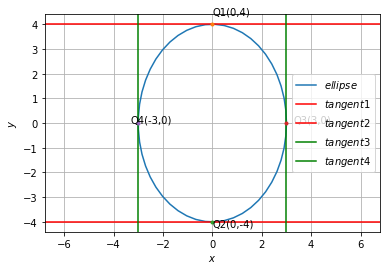
\includegraphics[width=\columnwidth]{./solutions/conics/1/16/ellipse.png}
	\caption{Figure depicting point of contact of tangents of ellipse parallel to x-axis and y-axis}
	\label{eq:solutions/1/16/fig1}
\end{figure}

\subsection{Solution.a)}
%\renewcommand{\theequation}{\theenumi}
\begin{enumerate}[label=\thesection.\arabic*.,ref=\thesection.\theenumi]
%\numberwithin{equation}{enumi}

%
\item from the $\Delta APB$ and $\Delta{AQB}$... 
%
\begin{align}
\norm{\vec{A-P}} = \norm{\vec{A-P}}
\\
\angle{AQB} = \angle{APB}
\end{align}
\\
$\vec{AB}$ is bisector of $\angle QAP$
\begin{align}
\implies\angle{AQB} = \angle{APB}
\end{align}
\\
thus from ASA conguransy
 
 \begin{align}
 \Delta APB \cong \Delta AQB
 \end{align}
\end{enumerate}

\subsection{Solution.b)}
%\renewcommand{\theequation}{\theenumi}
\begin{enumerate}[label=\thesection.\arabic*.,ref=\thesection.\theenumi]
%\numberwithin{equation}{enumi}
	
\item
from equation $\left(3.1.4\right)$...
\begin{align}
\Delta APB \cong \Delta AQB
\\
\implies\norm{\vec{BQ}} = \norm{\vec{BP}}
\end{align}


Hence proved

\end{enumerate}

%\subsection{Sol.c)}
%$\triangle ACB$ and $\triangle DCB$ are congruent to each other in SAS congruency.
\\
(i)Both the triangles have a common base , a.
\newline
(ii)AC = DB by using distance formula
\newline
(iii)$\angle ACB$ = $\angle DBC$ = 90$^{\circ}$ [ From Solution b)]
\\
Hence, proved.

%\subsection{Sol.d)}
%Since $\vec{CM}$ is halfway of $\vec{CD}$
\newline
$\norm{\vec{CM}}=\norm{\vec{CD}}$
\newline
From Solution b) it is clear that $\norm{\vec{CD}}=\norm{\vec{BA}}$
\newline
Therefore $\norm{\vec{CM}}=\frac{1}{2}\norm{\vec{AB}}$
\\
Hence, proved.



\end{document}


